\documentclass[12pt,a4paper]{article}
\usepackage[utf8]{inputenc}
\usepackage[russian]{babel}
\usepackage[OT1]{fontenc}
\usepackage{amsmath}
\usepackage{amsfonts}
\usepackage{amssymb}
\usepackage{graphicx}
\graphicspath{{Images/}}
\usepackage[left=2cm,right=2cm,top=2cm,bottom=2cm]{geometry}
\usepackage{calc}
\usepackage{wrapfig}
\usepackage{setspace}
\usepackage{indentfirst}
\usepackage{subfigure}
\usepackage{multirow}


\title{
Отчет о выполнении лабораторной работы 2.3.1 А

Получение и измерение вакуума
}

\author{Варламов Антоний, группа Б02-928}

\begin{document}

\maketitle

\newpage


	
	\newpage
	
	\section{Схема установки}
	\begin{figure}[h!]
		\begin{center}
			\begin{minipage}[h]{0.4\linewidth}
				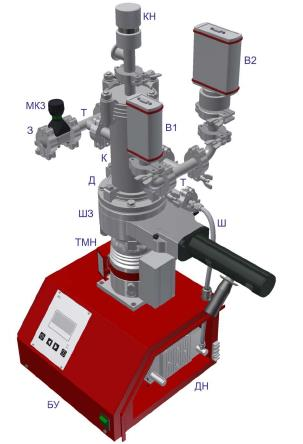
\includegraphics[width=1\linewidth]{scem_of_facility_front}
				\caption{Внешний вид установки. Вид спереди} %% подпись к рисунку
				\label{fig:scem_of_facility_front} %% метка рисунка для ссылки на него
			\end{minipage}
		\hfill
			\begin{minipage}[h]{0.4\linewidth}
				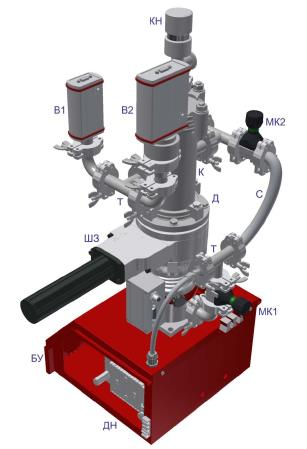
\includegraphics[width=1\linewidth]{scem_of_facility_rear}
				\caption{Внешний вид установки. Вид сзади}
				\label{fig:scem_of_facility_rear}
			\end{minipage}
		\end{center}
		\begin{center}
			\begin{minipage}[h]{0.7\linewidth}
				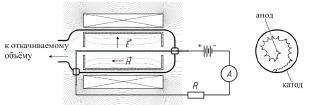
\includegraphics[width=1\linewidth]{Scem_of_vacuummetres}
				\caption{Принципиальная схема инверсно-магнетронного вакуумметра и траектории электронов в них}
				\label{fig:Scem_of_vacuummetres}
			\end{minipage}
		\end{center}
		\begin{center}
			\begin{minipage}[lh]{0.7\linewidth}
				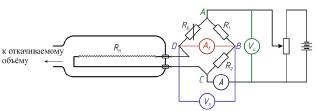
\includegraphics[width=1\linewidth]{Scem_of_vacuummetres_Pirani}
				\caption{Принципиальная схема терморезисторного вакуумметра (Пирани)} %% подпись к рисунку
				\label{fig:Scem_of_vacuummetres_Pirani} %% метка рисунка для ссылки на него
			\end{minipage}
		\hfill	
		\end{center}
	\end{figure}
	
	\newpage
	
	\begin{figure}[h!]
		\begin{center}
			\begin{minipage}[h]{0.4\linewidth}
				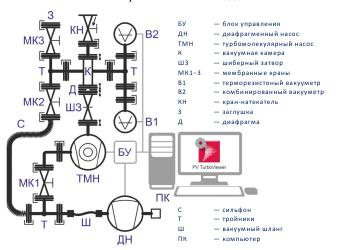
\includegraphics[width = 1.3\textwidth]{scem_of_facility}
				\caption{Cхема установки}
				\label{fig:scem_of_facility}
			\end{minipage}
		\hfill
			\begin{minipage}[h]{0.4\linewidth}
				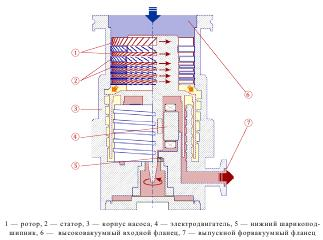
\includegraphics[width=1.25\linewidth]{Turbomolecular_pump_schem}
				\caption{Устройство турбомолекулярного насоса}
				\label{fig:Turbomolecular_pump_schem}
			\end{minipage}
		\end{center}
	\end{figure}
	
	На рисунках (\ref{fig:scem_of_facility_front}, \ref{fig:scem_of_facility_rear}) представлены изображения внешнего вида установки, на рисунках (\ref{fig:Scem_of_vacuummetres}, \ref{fig:Scem_of_vacuummetres_Pirani}) представлены принципиальные схемы вакуумметров, используемых в данной работе. На рисунках (\ref{fig:scem_of_facility}, \ref{fig:Turbomolecular_pump_schem}) представлена принципиальная схема установки и устройство турбомолекулярного насоса.
	
	
	\section{Теоретический материал}

	Одна из основных характеристик систем, работающих при вакууме -- число Кнудсена:
	
	\begin{equation}
		Kn = \frac{\lambda}{d}, 
	\end{equation}

	$\lambda$ -- длина свободного пробега молекул газа, $d$ -- характерный размер системы.
	
	В зависимости от значений числа Кнудсена определяют:
	
	1) низкий вакуум -- $Kn \ll 1$
	
	2) средний вакуум -- $Kn \sim 1$
	
	3) высокий вакуум -- $Kn \gg 1$
	
	Выпишем основные формулы, отображающие теоретические зависимости между исследуемыми величинами.
	
	
		Скорость откачки:
	\begin{equation}
		S = \frac{dV}{dt};
	\end{equation}	
	
		Падение давления:
	\begin{equation}
		\Delta P = P_{\text{вх}} - P_{\text{вых}};
	\end{equation}
		
		Пропускная способность:
	\begin{equation}
		U = \frac{Q}{\Delta P};
	\end{equation}
	
		Основное уравнение вакуумной механики:
	\begin{equation}
		\frac{1}{S_{0}} = \frac{1}{S_{text{н}}} + \frac{1}{U};
	\end{equation} 
	
	\begin{equation}
		Q_{\text{н}} = V\frac{P_{\text{к}} - P_{\text{н}}}{\Delta t}		
	\end{equation}
	
		Проводимость отверстия:
	\begin{equation}
		U_{\text{отв}} = \frac{1}{4} \pi R^{2} \sqrt{\frac{8kT}{\pi m}} \sim R^{2}\sqrt{T/m}
	\end{equation}
	
		Проводимость длинного трубопровода
	\begin{equation}
		U_{\text{тр}} = \frac{4}{3} \frac{R^{3}}{L} \sqrt{\frac{2\pi kT}{m}} \sim \frac{R^{3}}{L} \sqrt{\frac{T}{m}} 
	\end{equation}
	
		Уравнение откачки газа
	\begin{equation}
		P\left( t \right) = P_{1}\exp \left(- \frac{S_{0}}{V_{0}}t \right)
	\end{equation}
	
	
\section{Экспериментальная часть}

	\subsection{Определение откачиваемого объёма и измерение скорости откачки форвакуумным насосом}
	
	Для определения объемов частей установки (Объем вакуумной камеры -- $V_{K},$  объем форвакуумной магистрали + объем ТМН -- $V_{\text{ф.м. + тмн}}$ воспользуемся законом Бойля-Мариотта. Для этого необходимо определить давления в различном состоянии установки (Исследовать различные части установки).
	
	Для лучшей точности было проведено 3 измерения, результаты которых занесены в таблицу (\ref{tab:results_of_measuring_for_value}). Значения погрешностей определяются с помощью МНК.
	
	\begin{table}[h]
	\centering
		\begin{tabular}{|c|c|c|c|c|c|}
		\hline
		\multicolumn{2}{|c|}{1} & \multicolumn{2}{c|}{2} & \multicolumn{2}{c|}{3} \\ \hline
		p, mbar  & $\sigma_{p}$, mbar & p, mbar & $\sigma_{p}$, mbar & p, mbar & $\sigma_{p}$, mbar \\ \hline
		3,32     & 0,08         & 3,26    & 0,06         & 3,05    & 0,08         \\ \hline
		193      & 9            & 185     & 5            & 188     & 5            \\ \hline
		140      & 4            & 132     & 4            & 132     & 4            \\ \hline
		\end{tabular}
		\caption{Результаты измерения давления при различных конфигурациях системы.}
		\label{tab:results_of_measuring_for_value}
	\end{table}
	
	
	
	Используя закон Бойля-Мариотта получаем соотношения:
	
	\begin{equation}
		V_{K} = \frac{p_{\text{атм}} - p_{2}}{p_{2} - p_{1}} V_{\text{сильф}};
		\label{eq:value_of_vacuum_cam}
	\end{equation}
	
	\begin{equation}
		V_{\text{ф.м. + тмн}} = \frac{ \left( p_{3} - p_{2}\right) \left( V_{K} + V_{\text{сильф}}\right) }{p_{1} - p_{3}};
		\label{eq:value_of_forvacuum_tube}
	\end{equation}
	
	Используя соотношения (\ref{eq:value_of_vacuum_cam}, \ref{eq:value_of_forvacuum_tube}) определим объемы составных частей установки, а также погрешности косвенных измерений данных величин. Значения занесем в таблицу (\ref{tab:resultsof_measuring_for_diffrent_part_value}).
	
	\begin{table}[h]
		\centering
		\begin{tabular}{|c|c|c|c|c|c|}
		\hline
		номер измерения & $V_{C}, cm^{3}$ & $V_{K}, cm^{3}$ & $\sigma_{V_{K}}, cm^{3}$ & $V_{\text{ф.м. + тмн}}, cm^{3}$ & $\sigma_{V_{\text{ф.м. + тмн}}}, cm^{3}$ \\ \hline
		1               & 265             & 1140            & 60                       & 550                             & 25                                       \\ \hline
		2               & 265             & 1120            & 40                       & 575                      & 25                                       \\ \hline
		3               & 265             & 1120            & 40                       & 600                             & 25                                       \\ \hline
		\end{tabular}
		\caption{Результаты измерения объемов составных частей установки с погрешностью косвенного измерения}
		\label{tab:resultsof_measuring_for_diffrent_part_value}
	\end{table}
	
	Перейдем к оценке эффективной скорости откачки системы форвакуумным насосом в области, где она почти постоянна. Для этого построим зависимость $\ln (p) $ от $t$. График данной зависимости приведен на рисунке (\ref{fig:Depends_preasure_of_time}).

	
	\begin{figure}[h!]
		\begin{center}
			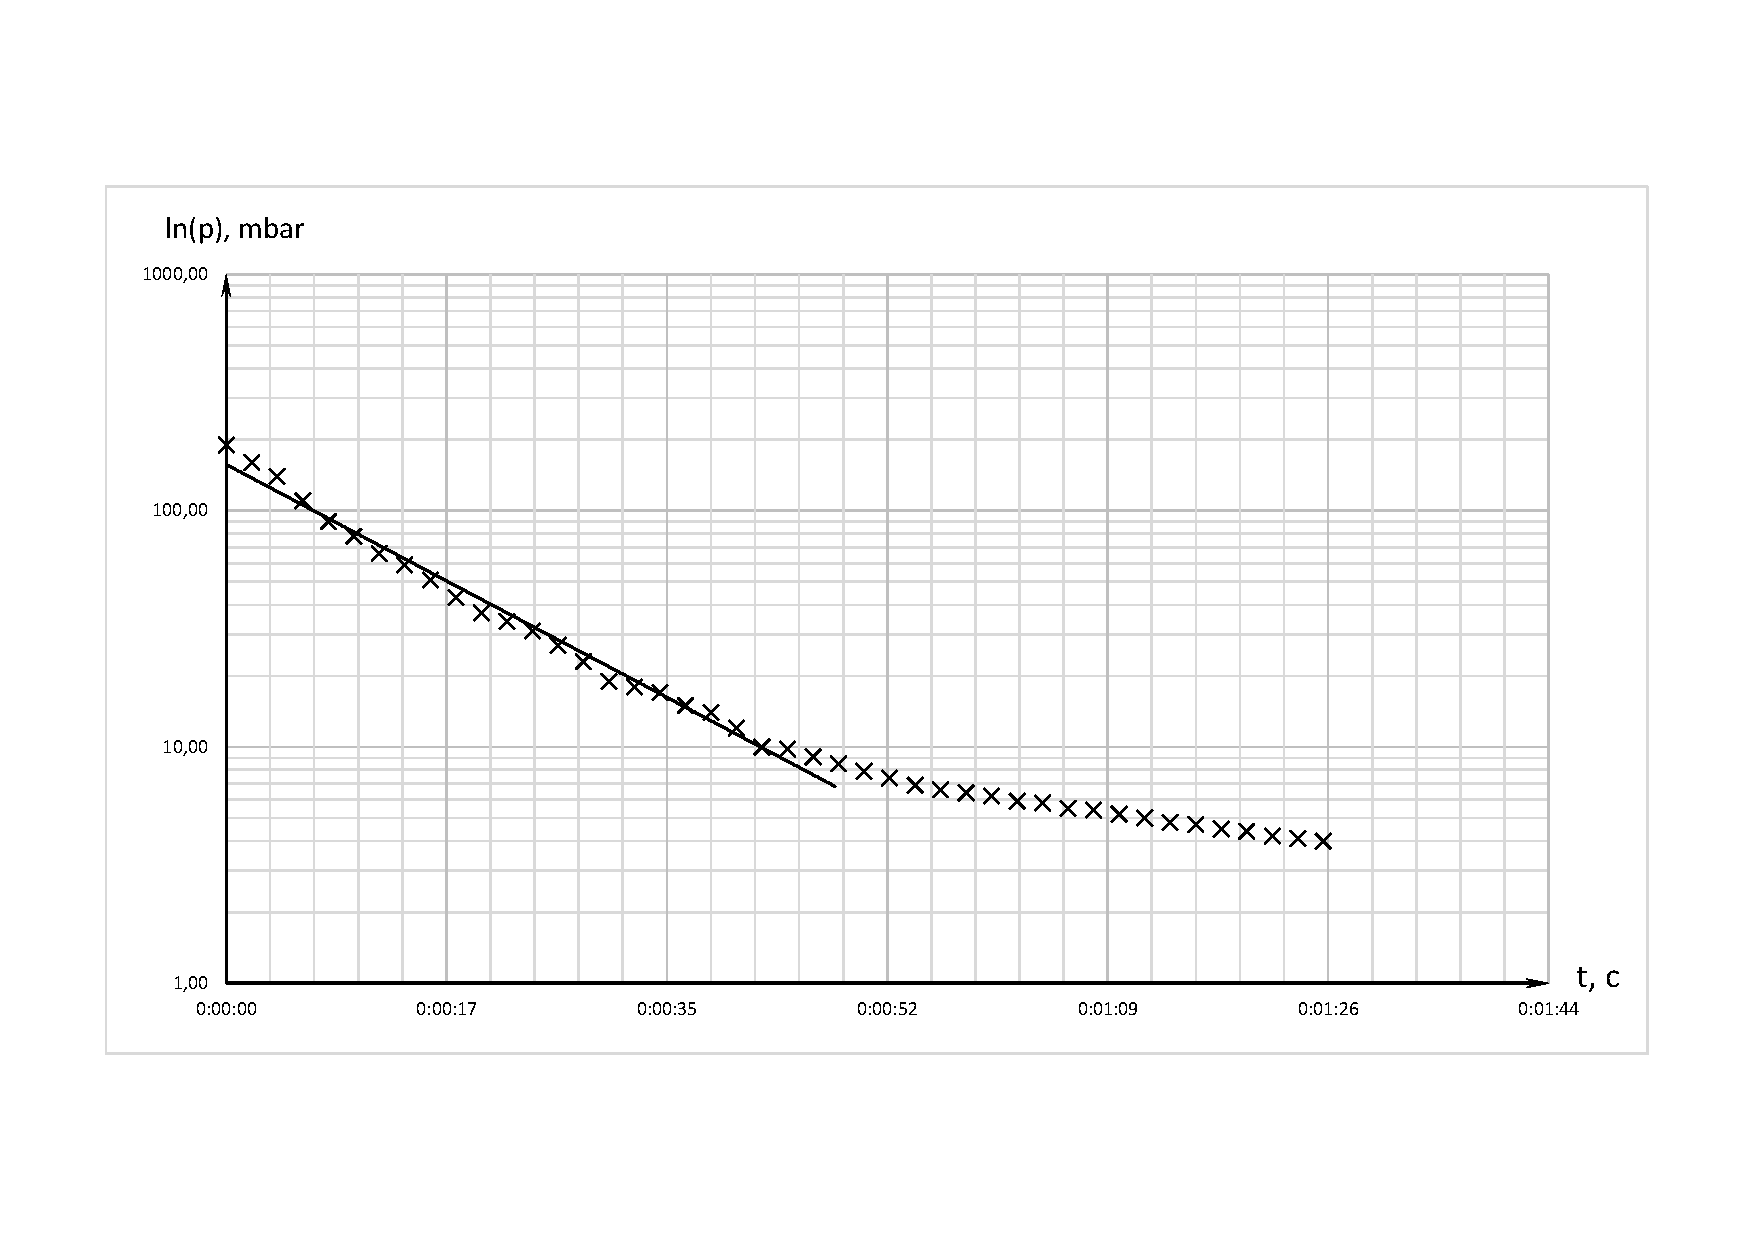
\includegraphics[width = 0.95\textwidth]{Depends_preasure_of_time}
			\caption{График зависимости $\ln (p) $ от $t$}
			\label{fig:Depends_preasure_of_time}
		\end{center}
	\end{figure}
	
	Линейному участку на данном графике соответствует значение $$\tau = 5 700 \pm 300\quad \text{mbar}\cdot\text{с}^{-1}$$.
	
	Определяя по этим данным рассчитаем эффективную скорость откачки:
	
	$$S_{0} = 0,66 \pm 0.12 \quad \frac{\text{м}^{3}}{\text{ч}}$$
	
	
	
	\subsection{Измерение скорости откачки турбомолекулярным насосом и определение предельного вакуума}
	
	Перейдем к определению скорости откачки турбомолекулярным насосом. Аналогично с предыдущим пунктом, построим график зависимости $\ln (p) $ от $t$. Данный график изображен на рисунке (\ref{fig:Depends_preasure_of_time_tmn}).
	
	Для турбомолекулярного насоса на линейном участке $$\tau = 350 \pm 30\quad \text{mbar}\cdot\text{с}^{-1}$$.
	
	\begin{figure}[h!]
		\begin{center}
			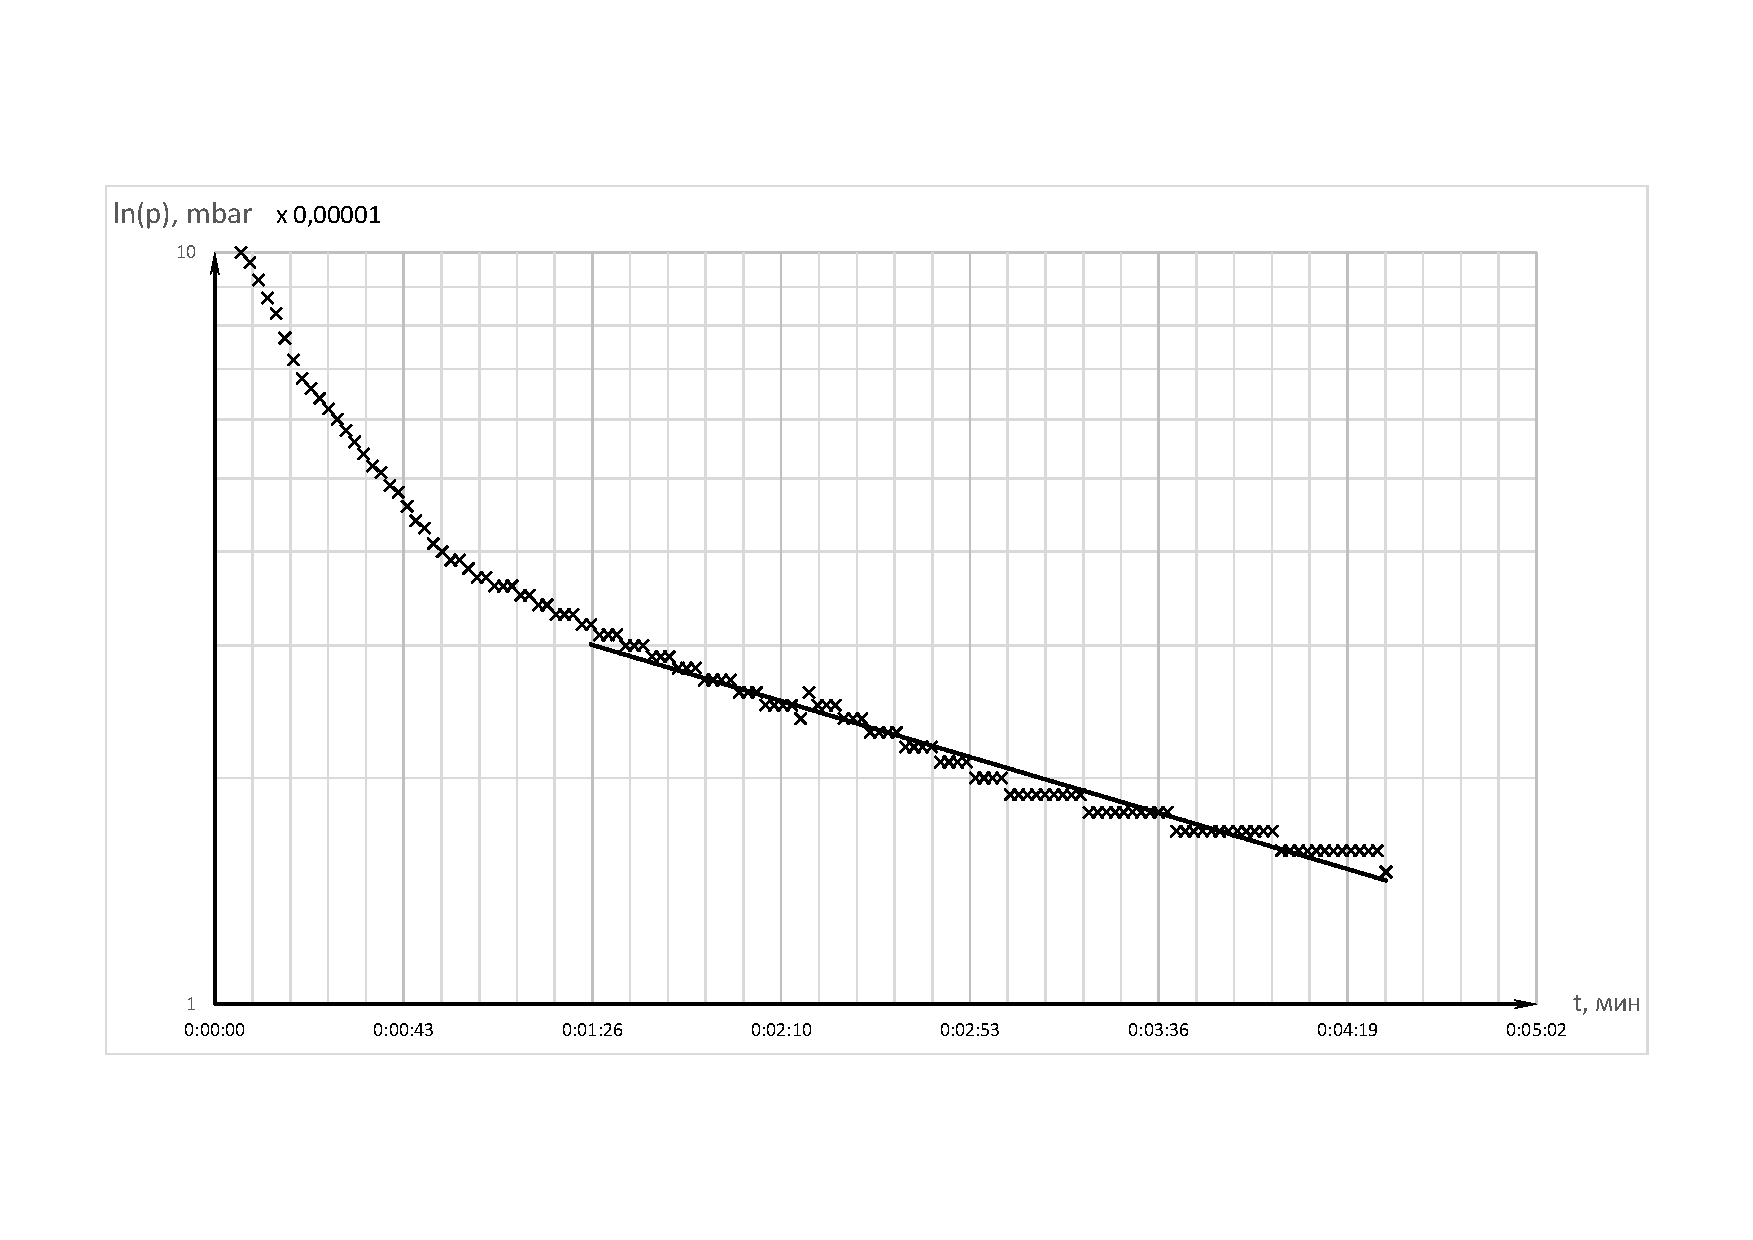
\includegraphics[width = 0.9\textwidth]{Depends_preasure_of_time_tmn}
			\caption{График зависимости $\ln (p) $ от $t$}
			\label{fig:Depends_preasure_of_time_tmn}
		\end{center}
	\end{figure}	
	
	Определение эффективной скорости откачки затруднительно, так как была допущена ошибка в ходе выполнения работы (Не получены данные для определения объема ТМН).
	
	\subsection{Создание искусственной течи и определение давления перехода в молекулярный режим}
	
	Построим график зависимости натекания от времени.
	
	\begin{figure}[h!]
		\begin{center}
			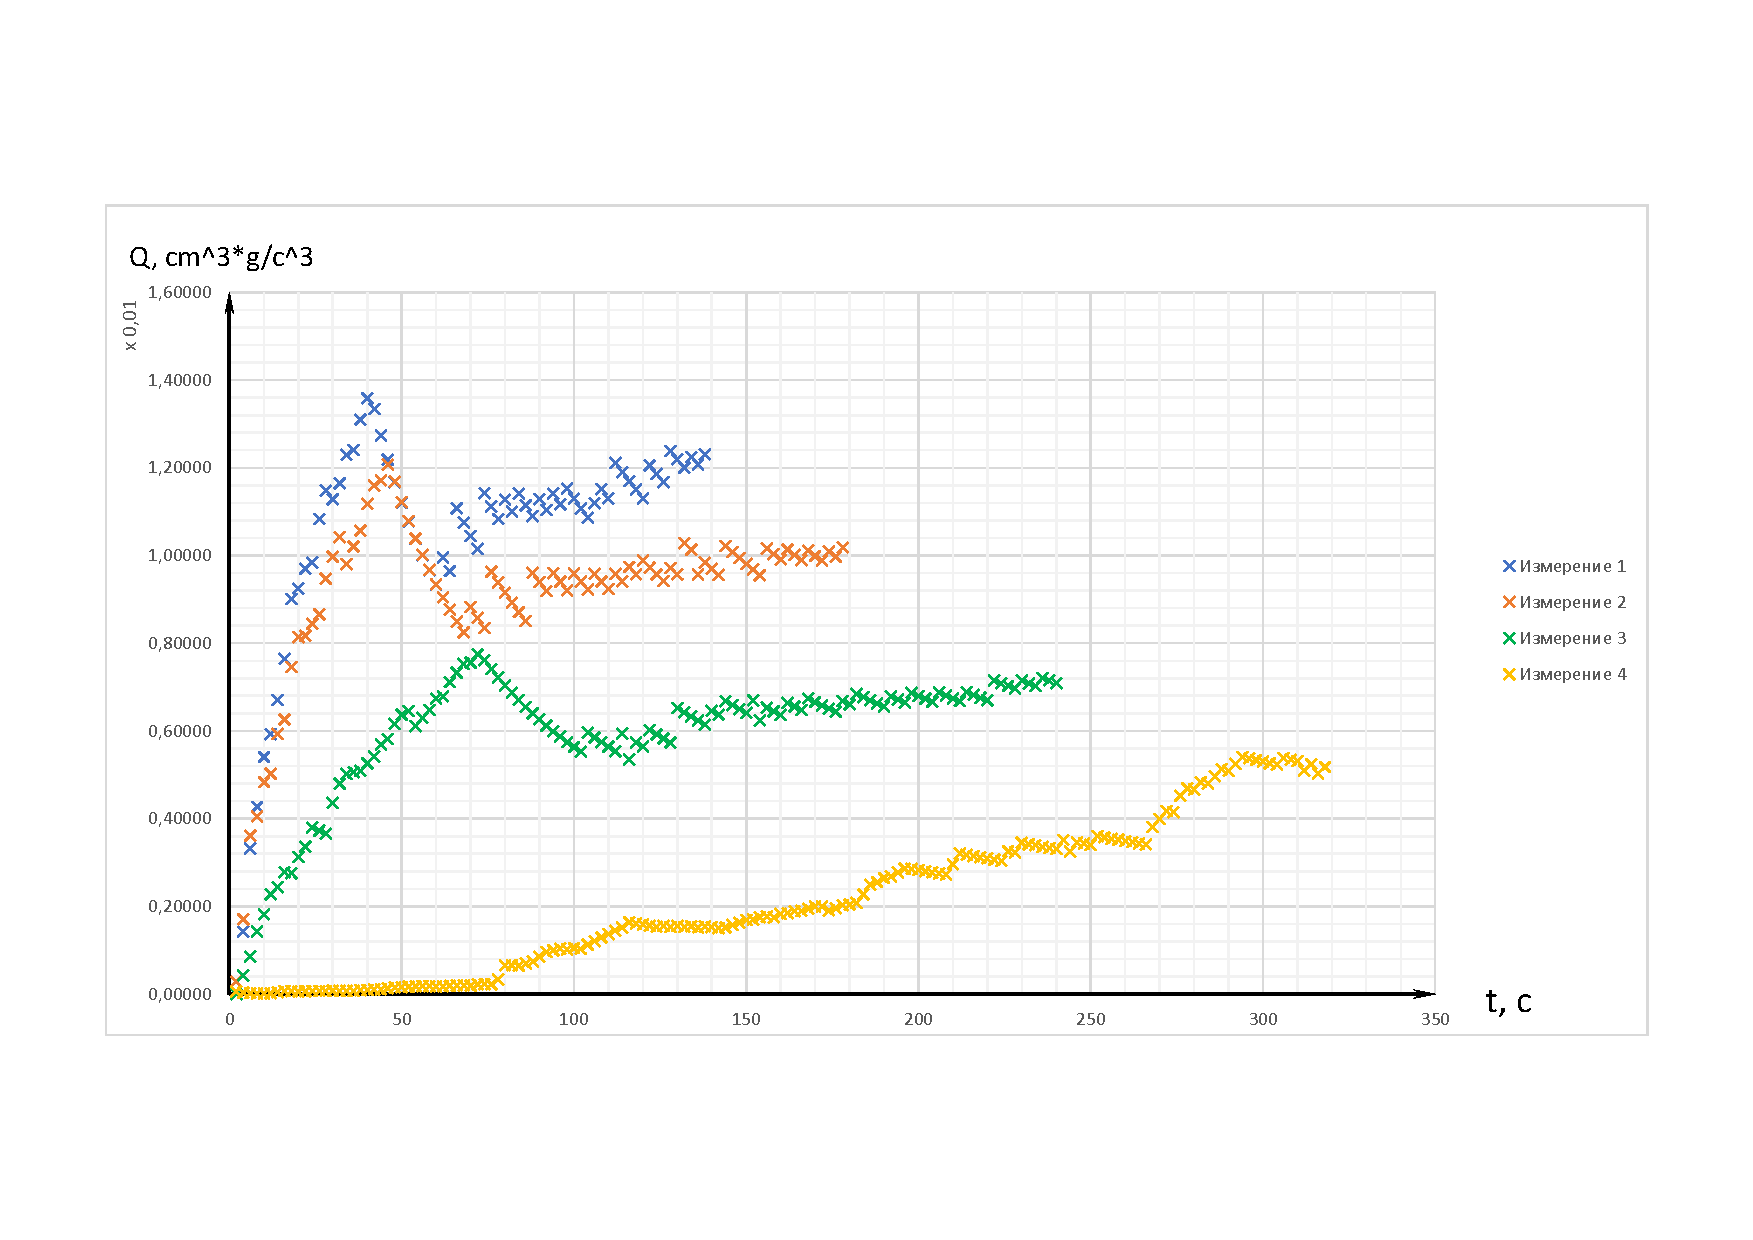
\includegraphics[width = 0.7\textwidth]{Natekanie}
			\caption{График зависимости $Q_{\text{н}} $ от $t$}
			\label{fig:Natekanie}
		\end{center}
	\end{figure}	
	
	Как видно из рисунка (\ref{fig:Natekanie}) сохранить слабый режим натекания удалось только в 4 измерении, в котором время повышения давления оказалось максимальным. Обусловлено это тем, что только в 4 измерении было достигнуто предельное давление, из-за чего на раннем этапе процесса натекание имело линейный характер.
	
\section{Исследование зависимости мощности турбины насоса от давления в камере}

	Построим график зависимости $p(W)$ в диапазоне предельных давлений. Данный график изображен на рисунке (\ref{fig:Depence_preasure_of_power}).
	
	
	
	\begin{figure}[h!]
		\begin{center}
			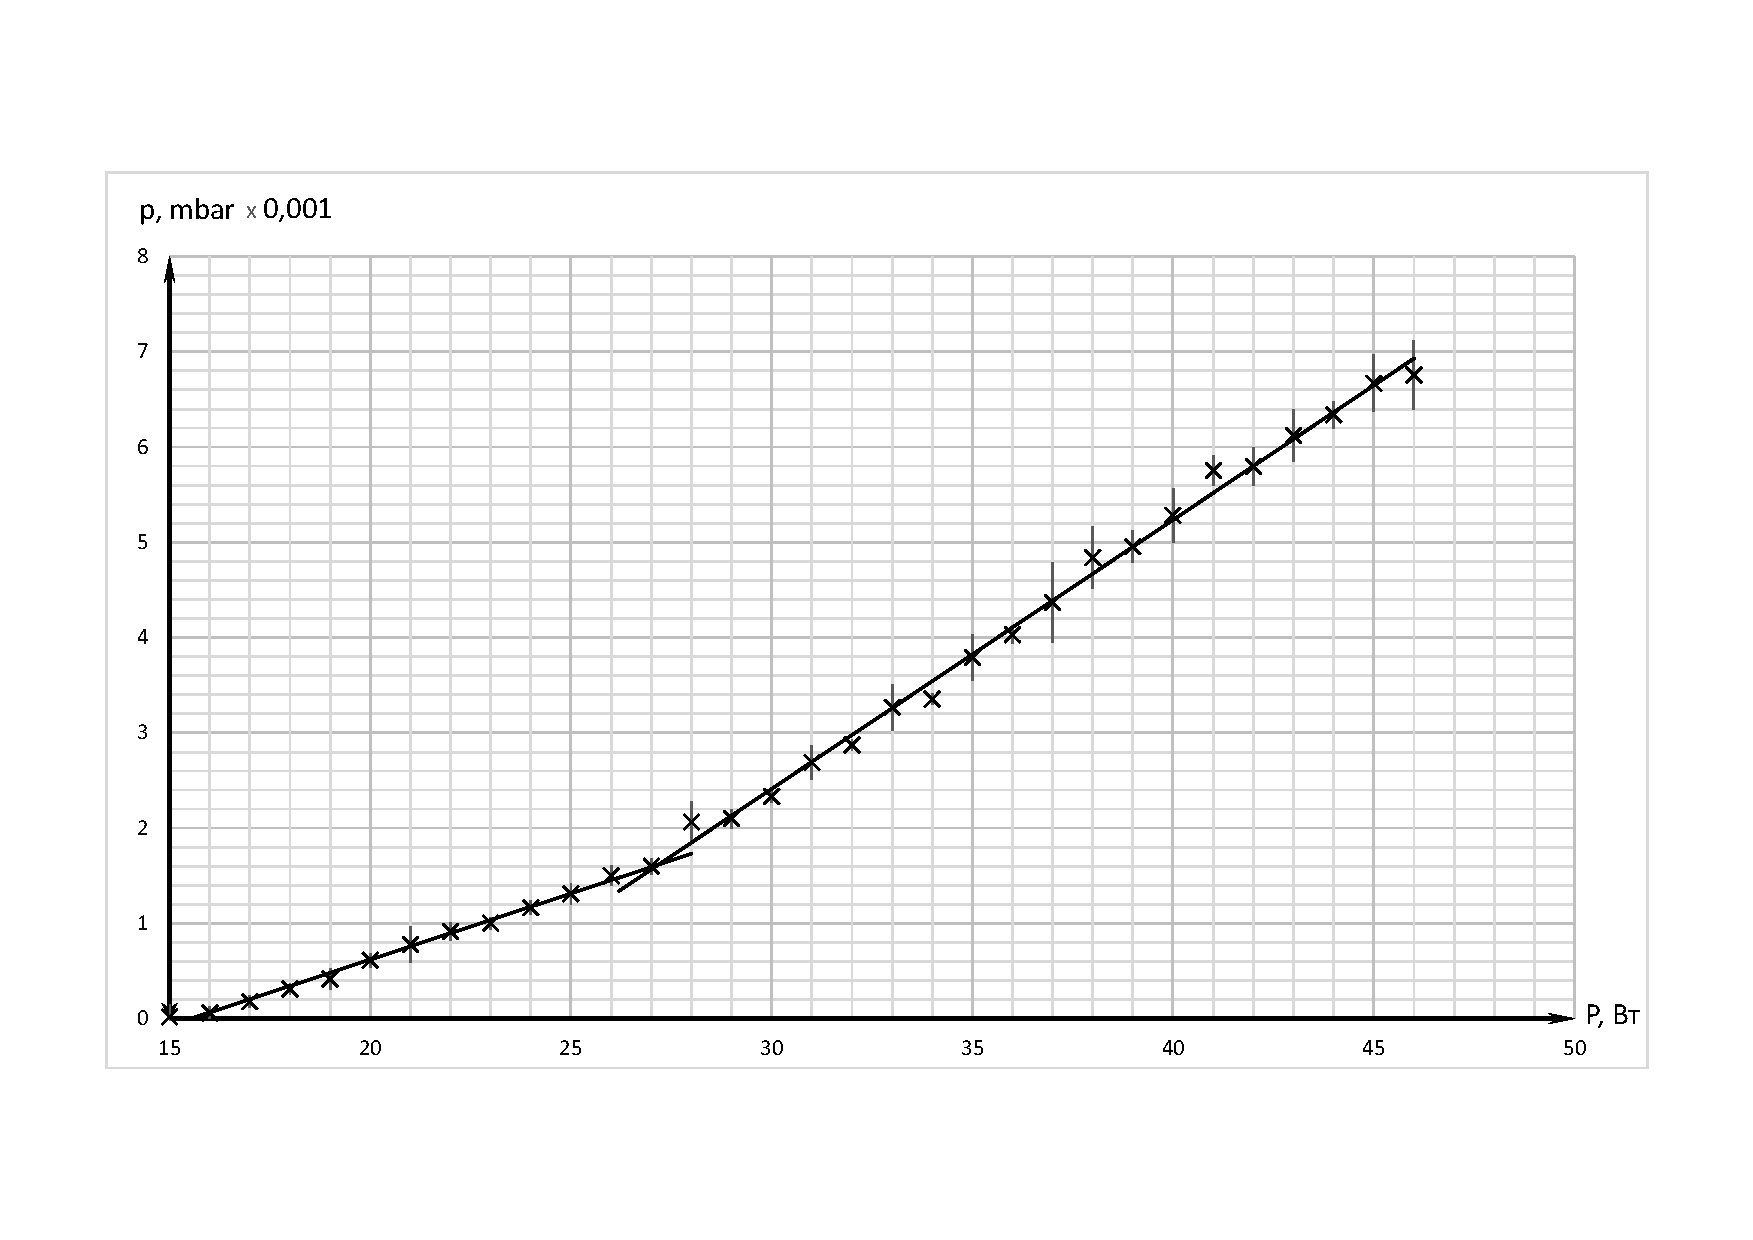
\includegraphics[width = 0.95\textwidth]{Depence_preasure_of_power}
			\caption{График зависимости $p$ от $W$}
			\label{fig:Depence_preasure_of_power}
		\end{center}
	\end{figure}
	
	Как видно из графика, полученная зависимость имеет линейный характер с характерным переходным процессом. Данный переходный процесс можно считать моментом перехода в молекулярный режим течения газа. Характерной особенностью данной зависимости является линейность даже при предельно больших давлениях, что противоречит имеющимся теоретическим предположениям. Кроме того, стоит отметить отношение угловых коэффициентов для аппроксимирующих прямых. Данное отношение равно $k = \frac{3,458}{1,096} \approx 3,5$.
	
	Давление, при котором происходит переход в молекулярный режим течения: $\sim 1,5 \cdot 10^{-6} bar$. при данном давлении мощность турбины насоса составляла 27-28 Вт. Наглядно просматривается зависимость эффективности работы турбомолекулярного насоса от предельного давления в камере насоса.
	
	
\section{Выводы}

\begin{enumerate}
	\item С приемлемой точностью были определены объемы составных частей установки:
	
	$$V_{K} = 1140 \pm 60 \quad \text{см}^3; \varepsilon_{V_{K}} = 0,052;$$
	
	$$V_{ф.м. + тмн} = 575 \pm 25 \quad \text{см}^3; \varepsilon_{V_{ф.м. + тмн}} = 0,043;$$
	
	Основной вклад в погрешность составляет погрешность косвенного измерения, так как при вычислении данных величин использовались зависимости от нескольких величин, имеющих погрешность прямого измерения. Погрешности входящих в итоговую формулу величин мало отличаются друг от другу (по порядку величины).
	
	Не удалось вычислить объем турбомолекулярного насоса, так как было допущена ошибка во время выполнения работы. (Пропущена один шаг в последовательности действий)
	
	\item Подтверждено большинство теоретических зависимостей, исследуемых в данной работе. все результаты укладываются в рассчитанные значения с учетом погрешности.
	
	\item Не удалось получить теоретическую зависимость давления от мощности турбомолекулярного насоса в области низких давлений. наблюдается линейность процесса, что противоречит теории, однако подтвержден переход в молекулярный режим течения газа при откачке.
	
	\item Все вычисленные погрешности не превосходят 30$\%$ от рассчитанных величин. Максимальная погрешность наблюдается в опыте по измерению скорости эффективной откачки. Основной вклад в данную погрешность внес коэффициент, определенный с помощью метода МНК по экспериментальным данным. Погрешность определения коэффициента -- $\varepsilon_{k} = 0,09$, что при использовании данной величины в косвенных измерениях сильно понижает точность определения величин.
\end{enumerate}

\end{document}